\documentclass[twoside]{book}

% Packages required by doxygen
\usepackage{fixltx2e}
\usepackage{calc}
\usepackage{doxygen}
\usepackage[export]{adjustbox} % also loads graphicx
\usepackage{graphicx}
\usepackage[utf8]{inputenc}
\usepackage{makeidx}
\usepackage{multicol}
\usepackage{multirow}
\PassOptionsToPackage{warn}{textcomp}
\usepackage{textcomp}
\usepackage[nointegrals]{wasysym}
\usepackage[table]{xcolor}

% Font selection
\usepackage[T1]{fontenc}
\usepackage[scaled=.90]{helvet}
\usepackage{courier}
\usepackage{amssymb}
\usepackage{sectsty}
\renewcommand{\familydefault}{\sfdefault}
\allsectionsfont{%
  \fontseries{bc}\selectfont%
  \color{darkgray}%
}
\renewcommand{\DoxyLabelFont}{%
  \fontseries{bc}\selectfont%
  \color{darkgray}%
}
\newcommand{\+}{\discretionary{\mbox{\scriptsize$\hookleftarrow$}}{}{}}

% Page & text layout
\usepackage{geometry}
\geometry{%
  a4paper,%
  top=2.5cm,%
  bottom=2.5cm,%
  left=2.5cm,%
  right=2.5cm%
}
\tolerance=750
\hfuzz=15pt
\hbadness=750
\setlength{\emergencystretch}{15pt}
\setlength{\parindent}{0cm}
\setlength{\parskip}{0.2cm}
\makeatletter
\renewcommand{\paragraph}{%
  \@startsection{paragraph}{4}{0ex}{-1.0ex}{1.0ex}{%
    \normalfont\normalsize\bfseries\SS@parafont%
  }%
}
\renewcommand{\subparagraph}{%
  \@startsection{subparagraph}{5}{0ex}{-1.0ex}{1.0ex}{%
    \normalfont\normalsize\bfseries\SS@subparafont%
  }%
}
\makeatother

% Headers & footers
\usepackage{fancyhdr}
\pagestyle{fancyplain}
\fancyhead[LE]{\fancyplain{}{\bfseries\thepage}}
\fancyhead[CE]{\fancyplain{}{}}
\fancyhead[RE]{\fancyplain{}{\bfseries\leftmark}}
\fancyhead[LO]{\fancyplain{}{\bfseries\rightmark}}
\fancyhead[CO]{\fancyplain{}{}}
\fancyhead[RO]{\fancyplain{}{\bfseries\thepage}}
\fancyfoot[LE]{\fancyplain{}{}}
\fancyfoot[CE]{\fancyplain{}{}}
\fancyfoot[RE]{\fancyplain{}{\bfseries\scriptsize Generated on Wed Jul 8 2015 09\+:52\+:12 for R\+C Car by Doxygen }}
\fancyfoot[LO]{\fancyplain{}{\bfseries\scriptsize Generated on Wed Jul 8 2015 09\+:52\+:12 for R\+C Car by Doxygen }}
\fancyfoot[CO]{\fancyplain{}{}}
\fancyfoot[RO]{\fancyplain{}{}}
\renewcommand{\footrulewidth}{0.4pt}
\renewcommand{\chaptermark}[1]{%
  \markboth{#1}{}%
}
\renewcommand{\sectionmark}[1]{%
  \markright{\thesection\ #1}%
}

% Indices & bibliography
\usepackage{natbib}
\usepackage[titles]{tocloft}
\setcounter{tocdepth}{3}
\setcounter{secnumdepth}{5}
\makeindex

% Hyperlinks (required, but should be loaded last)
\usepackage{ifpdf}
\ifpdf
  \usepackage[pdftex,pagebackref=true]{hyperref}
\else
  \usepackage[ps2pdf,pagebackref=true]{hyperref}
\fi
\hypersetup{%
  colorlinks=true,%
  linkcolor=blue,%
  citecolor=blue,%
  unicode%
}

% Custom commands
\newcommand{\clearemptydoublepage}{%
  \newpage{\pagestyle{empty}\cleardoublepage}%
}


%===== C O N T E N T S =====

\begin{document}

% Titlepage & ToC
\hypersetup{pageanchor=false,
             bookmarks=true,
             bookmarksnumbered=true,
             pdfencoding=unicode
            }
\pagenumbering{roman}
\begin{titlepage}
\vspace*{7cm}
\begin{center}%
{\Large R\+C Car }\\
\vspace*{1cm}
{\large Generated by Doxygen 1.8.10}\\
\vspace*{0.5cm}
{\small Wed Jul 8 2015 09:52:12}\\
\end{center}
\end{titlepage}
\clearemptydoublepage
\tableofcontents
\clearemptydoublepage
\pagenumbering{arabic}
\hypersetup{pageanchor=true}

%--- Begin generated contents ---
\chapter{Data Structure Index}
\section{Data Structures}
Here are the data structures with brief descriptions\+:\begin{DoxyCompactList}
\item\contentsline{section}{\hyperlink{struct____freelist}{\+\_\+\+\_\+freelist} }{\pageref{struct____freelist}}{}
\item\contentsline{section}{\hyperlink{struct_a_c_m_functional_descriptor}{A\+C\+M\+Functional\+Descriptor} }{\pageref{struct_a_c_m_functional_descriptor}}{}
\item\contentsline{section}{\hyperlink{struct_c_d_c_c_s_interface_descriptor}{C\+D\+C\+C\+S\+Interface\+Descriptor} }{\pageref{struct_c_d_c_c_s_interface_descriptor}}{}
\item\contentsline{section}{\hyperlink{struct_c_d_c_c_s_interface_descriptor4}{C\+D\+C\+C\+S\+Interface\+Descriptor4} }{\pageref{struct_c_d_c_c_s_interface_descriptor4}}{}
\item\contentsline{section}{\hyperlink{struct_c_d_c_descriptor}{C\+D\+C\+Descriptor} }{\pageref{struct_c_d_c_descriptor}}{}
\item\contentsline{section}{\hyperlink{class_client}{Client} }{\pageref{class_client}}{}
\item\contentsline{section}{\hyperlink{struct_c_m_functional_descriptor}{C\+M\+Functional\+Descriptor} }{\pageref{struct_c_m_functional_descriptor}}{}
\item\contentsline{section}{\hyperlink{struct_config_descriptor}{Config\+Descriptor} }{\pageref{struct_config_descriptor}}{}
\item\contentsline{section}{\hyperlink{struct_device_descriptor}{Device\+Descriptor} }{\pageref{struct_device_descriptor}}{}
\item\contentsline{section}{\hyperlink{struct_endpoint_descriptor}{Endpoint\+Descriptor} }{\pageref{struct_endpoint_descriptor}}{}
\item\contentsline{section}{\hyperlink{class_hardware_serial}{Hardware\+Serial} }{\pageref{class_hardware_serial}}{}
\item\contentsline{section}{\hyperlink{struct_h_i_d_desc_descriptor}{H\+I\+D\+Desc\+Descriptor} }{\pageref{struct_h_i_d_desc_descriptor}}{}
\item\contentsline{section}{\hyperlink{struct_h_i_d_descriptor}{H\+I\+D\+Descriptor} }{\pageref{struct_h_i_d_descriptor}}{}
\item\contentsline{section}{\hyperlink{struct_i_a_d_descriptor}{I\+A\+D\+Descriptor} }{\pageref{struct_i_a_d_descriptor}}{}
\item\contentsline{section}{\hyperlink{struct_interface_descriptor}{Interface\+Descriptor} }{\pageref{struct_interface_descriptor}}{}
\item\contentsline{section}{\hyperlink{class_i_p_address}{I\+P\+Address} }{\pageref{class_i_p_address}}{}
\item\contentsline{section}{\hyperlink{struct_m_s_c_descriptor}{M\+S\+C\+Descriptor} }{\pageref{struct_m_s_c_descriptor}}{}
\item\contentsline{section}{\hyperlink{struct_stream_1_1_multi_target}{Stream\+::\+Multi\+Target} }{\pageref{struct_stream_1_1_multi_target}}{}
\item\contentsline{section}{\hyperlink{structport__types__struct}{port\+\_\+types\+\_\+struct} \\*New datatype used in table which connects Logical Input Definitions to Physical Input Def }{\pageref{structport__types__struct}}{}
\item\contentsline{section}{\hyperlink{class_print}{Print} }{\pageref{class_print}}{}
\item\contentsline{section}{\hyperlink{class_printable}{Printable} }{\pageref{class_printable}}{}
\item\contentsline{section}{\hyperlink{class_server}{Server} }{\pageref{class_server}}{}
\item\contentsline{section}{\hyperlink{class_stream}{Stream} }{\pageref{class_stream}}{}
\item\contentsline{section}{\hyperlink{struct_task_type__st_type}{Task\+Type\+\_\+st\+Type} \\*Structure used to define a task and the interval of the execution }{\pageref{struct_task_type__st_type}}{}
\item\contentsline{section}{\hyperlink{class_u_d_p}{U\+D\+P} }{\pageref{class_u_d_p}}{}
\end{DoxyCompactList}

\chapter{File Index}
\section{File List}
Here is a list of all files with brief descriptions\+:\begin{DoxyCompactList}
\item\contentsline{section}{\hyperlink{_project_main_8cpp}{Project\+Main.\+cpp} }{\pageref{_project_main_8cpp}}{}
\item\contentsline{section}{\hyperlink{_project_main_8h}{Project\+Main.\+h} }{\pageref{_project_main_8h}}{}
\item\contentsline{section}{\hyperlink{scheduler_config_8h}{scheduler\+Config.\+h} }{\pageref{scheduler_config_8h}}{}
\end{DoxyCompactList}

\chapter{Data Structure Documentation}
\hypertarget{struct_task_type__st_type}{}\section{Task\+Type\+\_\+st\+Type Struct Reference}
\label{struct_task_type__st_type}\index{Task\+Type\+\_\+st\+Type@{Task\+Type\+\_\+st\+Type}}


{\ttfamily \#include $<$scheduler\+Config.\+h$>$}

\subsection*{Data Fields}
\begin{DoxyCompactItemize}
\item 
uint16\+\_\+t \hyperlink{struct_task_type__st_type_aa40544fbcdb815df9f6a9835488e484d}{interval\+\_\+u16}
\item 
void($\ast$ \hyperlink{struct_task_type__st_type_a86cfdbe6606dca2bdfa7ff9b37e9f9be}{ptr\+Func} )(void)
\end{DoxyCompactItemize}


\subsection{Detailed Description}
Struct Task\+Type Task\+Type structure is used to define the parameters required in order to configure a task. 

Definition at line 49 of file scheduler\+Config.\+h.



\subsection{Field Documentation}
\hypertarget{struct_task_type__st_type_aa40544fbcdb815df9f6a9835488e484d}{}\index{Task\+Type\+\_\+st\+Type@{Task\+Type\+\_\+st\+Type}!interval\+\_\+u16@{interval\+\_\+u16}}
\index{interval\+\_\+u16@{interval\+\_\+u16}!Task\+Type\+\_\+st\+Type@{Task\+Type\+\_\+st\+Type}}
\subsubsection[{interval\+\_\+u16}]{\setlength{\rightskip}{0pt plus 5cm}uint16\+\_\+t interval\+\_\+u16}\label{struct_task_type__st_type_aa40544fbcdb815df9f6a9835488e484d}


Definition at line 50 of file scheduler\+Config.\+h.

\hypertarget{struct_task_type__st_type_a86cfdbe6606dca2bdfa7ff9b37e9f9be}{}\index{Task\+Type\+\_\+st\+Type@{Task\+Type\+\_\+st\+Type}!ptr\+Func@{ptr\+Func}}
\index{ptr\+Func@{ptr\+Func}!Task\+Type\+\_\+st\+Type@{Task\+Type\+\_\+st\+Type}}
\subsubsection[{ptr\+Func}]{\setlength{\rightskip}{0pt plus 5cm}void($\ast$ ptr\+Func) (void)}\label{struct_task_type__st_type_a86cfdbe6606dca2bdfa7ff9b37e9f9be}


Definition at line 51 of file scheduler\+Config.\+h.



The documentation for this struct was generated from the following file\+:\begin{DoxyCompactItemize}
\item 
\hyperlink{scheduler_config_8h}{scheduler\+Config.\+h}\end{DoxyCompactItemize}

\chapter{File Documentation}
\hypertarget{_project_main_8cpp}{}\section{Arduino\+U\+N\+O/src/\+Project\+Files/\+Project\+Main.cpp File Reference}
\label{_project_main_8cpp}\index{Arduino\+U\+N\+O/src/\+Project\+Files/\+Project\+Main.\+cpp@{Arduino\+U\+N\+O/src/\+Project\+Files/\+Project\+Main.\+cpp}}


File containing functions for I\+O External.  


{\ttfamily \#include $<$Project\+Main.\+h$>$}\\*
{\ttfamily \#include $<$scheduler\+Config.\+h$>$}\\*
{\ttfamily \#include $<$P\+W\+M.\+h$>$}\\*
{\ttfamily \#include $<$avr/io.\+h$>$}\\*
{\ttfamily \#include $<$avr/interrupt.\+h$>$}\\*
{\ttfamily \#include \char`\"{}I\+O\+\_\+\+H\+A\+L/\+I\+O\+\_\+extern.\+h\char`\"{}}\\*
{\ttfamily \#include \char`\"{}A\+P\+P/lights/lights\+\_\+extern.\+h\char`\"{}}\\*
Include dependency graph for Project\+Main.\+cpp\+:\nopagebreak
\begin{figure}[H]
\begin{center}
\leavevmode
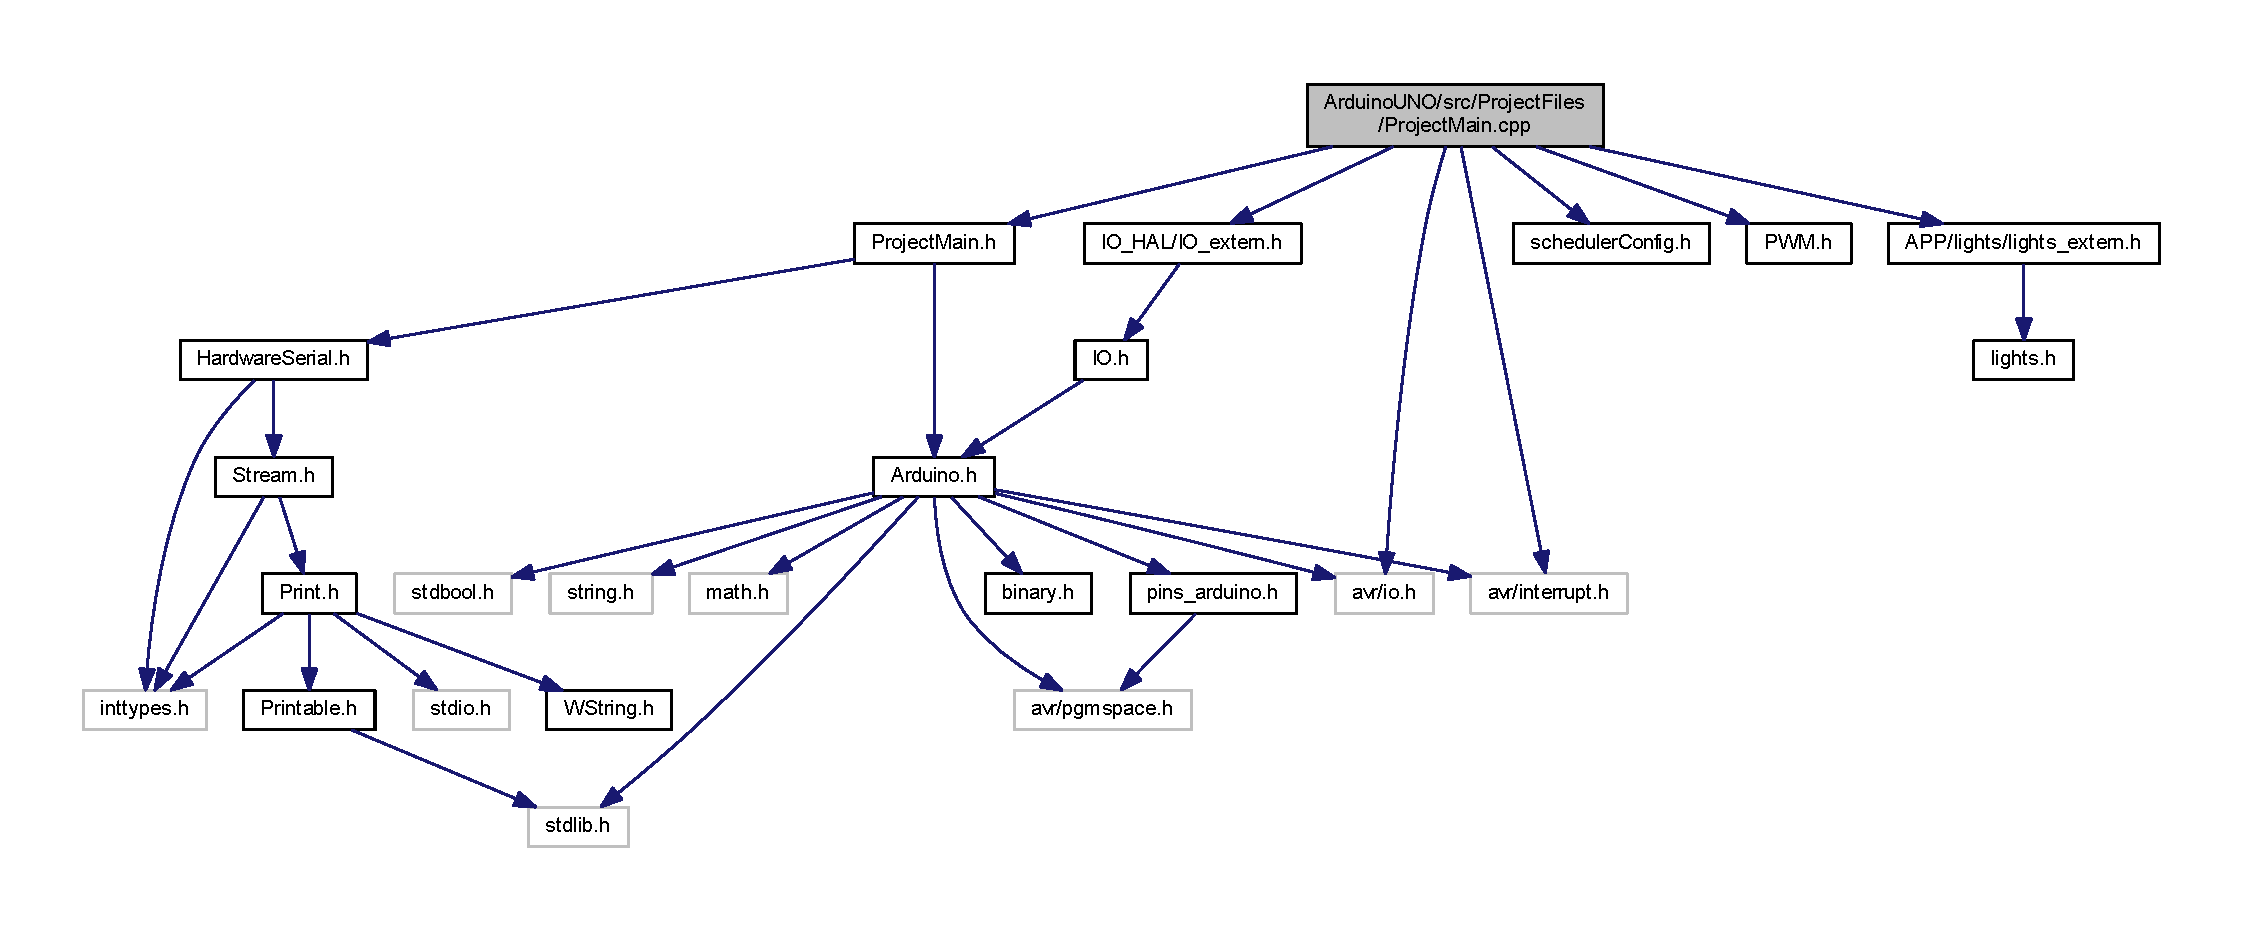
\includegraphics[width=350pt]{_project_main_8cpp__incl}
\end{center}
\end{figure}
\subsection*{Functions}
\begin{DoxyCompactItemize}
\item 
\hyperlink{struct_task_type__st_type}{Task\+Type\+\_\+st\+Type} $\ast$ \hyperlink{_project_main_8cpp_a612f7225aba66da17398c5472584559d}{task\+Get\+Config\+Ptr} (void)
\begin{DoxyCompactList}\small\item\em Implementation of the function that returns a pointer to the tasks array. \end{DoxyCompactList}\item 
uint8\+\_\+t \hyperlink{_project_main_8cpp_aac54e2201642d6b9c94f85ad2adbc7da}{get\+Nr\+Tasks} (void)
\begin{DoxyCompactList}\small\item\em Implementation of the function that returns the number of current tasks cheduled to run. \end{DoxyCompactList}\item 
void \hyperlink{_project_main_8cpp_a4fc01d736fe50cf5b977f755b675f11d}{setup} ()
\item 
void \hyperlink{_project_main_8cpp_afe461d27b9c48d5921c00d521181f12f}{loop} ()
\item 
void \hyperlink{_project_main_8cpp_aa0a2444ea9e75ec2a583b7e8a38560a6}{task20ms} (void)
\begin{DoxyCompactList}\small\item\em Implementation of function that handle the 20ms requests. \end{DoxyCompactList}\item 
void \hyperlink{_project_main_8cpp_aca27d12738aa55893e5242ed21ab789c}{task40ms} (void)
\begin{DoxyCompactList}\small\item\em Implementation of function that handle the 40ms requests. \end{DoxyCompactList}\item 
void \hyperlink{_project_main_8cpp_ada995e88886fe969d52c9f551201f7bc}{task60ms} (void)
\begin{DoxyCompactList}\small\item\em Implementation of function that handle the 60ms requests. \end{DoxyCompactList}\item 
void \hyperlink{_project_main_8cpp_abc513c77d3ae6919b5983e6564643c11}{task100ms} (void)
\begin{DoxyCompactList}\small\item\em Implementation of function that handle the 100ms requests. \end{DoxyCompactList}\item 
void \hyperlink{_project_main_8cpp_acf0bcd0e759358b9284f65e0a55bc193}{task1000ms} (void)
\begin{DoxyCompactList}\small\item\em Implementation of function that handle the 1000ms requests. \end{DoxyCompactList}\item 
void \hyperlink{_project_main_8cpp_a99eb04bf8fed2beecfb3cb74451416c5}{timer0\+\_\+init} ()
\begin{DoxyCompactList}\small\item\em Implementation of the function that initialize the timer0. \end{DoxyCompactList}\item 
void \hyperlink{_project_main_8cpp_abb302081b7dbd40d0fea4bbe53fd9b7b}{timer1\+\_\+init} ()
\begin{DoxyCompactList}\small\item\em Implementation of the function that initialize the timer1. \end{DoxyCompactList}\item 
\hyperlink{_project_main_8cpp_ab16889ae984b9b798989a0d239283cac}{I\+S\+R} (T\+I\+M\+E\+R1\+\_\+\+O\+V\+F\+\_\+vect)
\begin{DoxyCompactList}\small\item\em Implementation of the function that handle timer1 overflow I\+S\+R. \end{DoxyCompactList}\item 
void \hyperlink{_project_main_8cpp_af9ee60277083a5fd0fe10327f1b4eee7}{P\+W\+M\+\_\+\+Init} ()
\begin{DoxyCompactList}\small\item\em Implementation of the function that handle timer0 overflow I\+S\+R. \end{DoxyCompactList}\end{DoxyCompactItemize}
\subsection*{Variables}
\begin{DoxyCompactItemize}
\item 
uint8\+\_\+t \hyperlink{_project_main_8cpp_ad626e67a0337fbbad267d2ea8187a995}{stui\+\_\+\+Task\+Index}
\item 
volatile uint8\+\_\+t \hyperlink{_project_main_8cpp_a771478af671521a8cc845b8efbf0855e}{task\+Time\+Counter\+Flag\+\_\+u8}
\item 
volatile uint8\+\_\+t \hyperlink{_project_main_8cpp_aef920dc87f0a96b97b10da1251f9d821}{task\+Time\+Counter\+\_\+u8}
\item 
const uint8\+\_\+t \hyperlink{_project_main_8cpp_a364618e091f6af2a4ee81e8a38f2f974}{cui\+\_\+number\+Of\+Tasks} = \hyperlink{_project_main_8cpp_aac54e2201642d6b9c94f85ad2adbc7da}{get\+Nr\+Tasks}()
\end{DoxyCompactItemize}


\subsection{Detailed Description}
File containing functions for I\+O External. 

\begin{DoxyAuthor}{Author}
Adrian 
\end{DoxyAuthor}
\begin{DoxyDate}{Date}
26/05/2015 Here typically goes a more extensive explanation of what the header defines. Doxygens tags are words preceeded by either a backslash \textbackslash{} or by an at symbol @. 
\end{DoxyDate}
\begin{DoxySeeAlso}{See also}
\href{http://www.stack.nl/~dimitri/doxygen/docblocks.html}{\tt http\+://www.\+stack.\+nl/$\sim$dimitri/doxygen/docblocks.\+html} 

\href{http://www.stack.nl/~dimitri/doxygen/commands.html}{\tt http\+://www.\+stack.\+nl/$\sim$dimitri/doxygen/commands.\+html} 
\end{DoxySeeAlso}


\subsection{Function Documentation}
\hypertarget{_project_main_8cpp_aac54e2201642d6b9c94f85ad2adbc7da}{}\index{Project\+Main.\+cpp@{Project\+Main.\+cpp}!get\+Nr\+Tasks@{get\+Nr\+Tasks}}
\index{get\+Nr\+Tasks@{get\+Nr\+Tasks}!Project\+Main.\+cpp@{Project\+Main.\+cpp}}
\subsubsection[{get\+Nr\+Tasks(void)}]{\setlength{\rightskip}{0pt plus 5cm}uint8\+\_\+t get\+Nr\+Tasks (
\begin{DoxyParamCaption}
\item[{void}]{}
\end{DoxyParamCaption}
)}\label{_project_main_8cpp_aac54e2201642d6b9c94f85ad2adbc7da}


Implementation of the function that returns the number of current tasks cheduled to run. 

\begin{DoxyReturn}{Returns}
number of tasks 
\end{DoxyReturn}


Definition at line 79 of file Project\+Main.\+cpp.

\hypertarget{_project_main_8cpp_ab16889ae984b9b798989a0d239283cac}{}\index{Project\+Main.\+cpp@{Project\+Main.\+cpp}!I\+S\+R@{I\+S\+R}}
\index{I\+S\+R@{I\+S\+R}!Project\+Main.\+cpp@{Project\+Main.\+cpp}}
\subsubsection[{I\+S\+R(\+T\+I\+M\+E\+R1\+\_\+\+O\+V\+F\+\_\+vect)}]{\setlength{\rightskip}{0pt plus 5cm}I\+S\+R (
\begin{DoxyParamCaption}
\item[{T\+I\+M\+E\+R1\+\_\+\+O\+V\+F\+\_\+vect}]{}
\end{DoxyParamCaption}
)}\label{_project_main_8cpp_ab16889ae984b9b798989a0d239283cac}


Implementation of the function that handle timer1 overflow I\+S\+R. 

Implementation of the function that handle timer1 overflow I\+S\+R \begin{DoxyReturn}{Returns}
void 
\end{DoxyReturn}


Definition at line 239 of file Project\+Main.\+cpp.

\hypertarget{_project_main_8cpp_afe461d27b9c48d5921c00d521181f12f}{}\index{Project\+Main.\+cpp@{Project\+Main.\+cpp}!loop@{loop}}
\index{loop@{loop}!Project\+Main.\+cpp@{Project\+Main.\+cpp}}
\subsubsection[{loop()}]{\setlength{\rightskip}{0pt plus 5cm}void loop (
\begin{DoxyParamCaption}
\item[{void}]{}
\end{DoxyParamCaption}
)}\label{_project_main_8cpp_afe461d27b9c48d5921c00d521181f12f}


Definition at line 107 of file Project\+Main.\+cpp.



Here is the caller graph for this function\+:\nopagebreak
\begin{figure}[H]
\begin{center}
\leavevmode
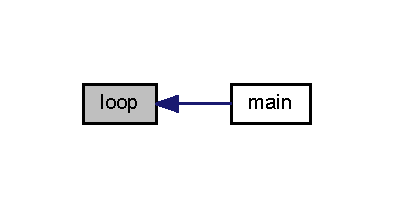
\includegraphics[width=189pt]{_project_main_8cpp_afe461d27b9c48d5921c00d521181f12f_icgraph}
\end{center}
\end{figure}


\hypertarget{_project_main_8cpp_af9ee60277083a5fd0fe10327f1b4eee7}{}\index{Project\+Main.\+cpp@{Project\+Main.\+cpp}!P\+W\+M\+\_\+\+Init@{P\+W\+M\+\_\+\+Init}}
\index{P\+W\+M\+\_\+\+Init@{P\+W\+M\+\_\+\+Init}!Project\+Main.\+cpp@{Project\+Main.\+cpp}}
\subsubsection[{P\+W\+M\+\_\+\+Init()}]{\setlength{\rightskip}{0pt plus 5cm}void P\+W\+M\+\_\+\+Init (
\begin{DoxyParamCaption}
{}
\end{DoxyParamCaption}
)}\label{_project_main_8cpp_af9ee60277083a5fd0fe10327f1b4eee7}


Implementation of the function that handle timer0 overflow I\+S\+R. 

Implementation of the function that handle timer0 overflow I\+S\+R \begin{DoxyReturn}{Returns}
void 
\end{DoxyReturn}


Definition at line 256 of file Project\+Main.\+cpp.

\hypertarget{_project_main_8cpp_a4fc01d736fe50cf5b977f755b675f11d}{}\index{Project\+Main.\+cpp@{Project\+Main.\+cpp}!setup@{setup}}
\index{setup@{setup}!Project\+Main.\+cpp@{Project\+Main.\+cpp}}
\subsubsection[{setup()}]{\setlength{\rightskip}{0pt plus 5cm}void setup (
\begin{DoxyParamCaption}
\item[{void}]{}
\end{DoxyParamCaption}
)}\label{_project_main_8cpp_a4fc01d736fe50cf5b977f755b675f11d}


Definition at line 93 of file Project\+Main.\+cpp.



Here is the call graph for this function\+:\nopagebreak
\begin{figure}[H]
\begin{center}
\leavevmode
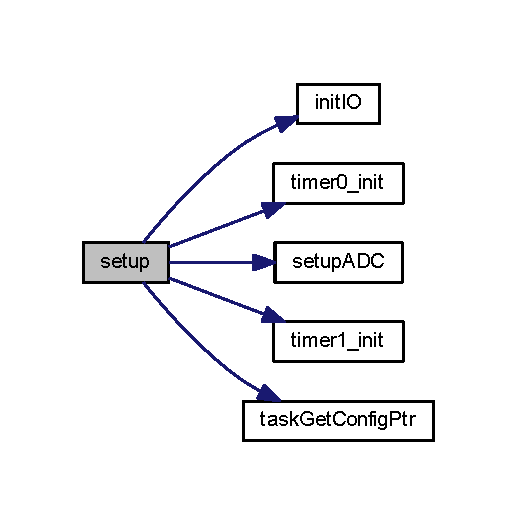
\includegraphics[width=248pt]{_project_main_8cpp_a4fc01d736fe50cf5b977f755b675f11d_cgraph}
\end{center}
\end{figure}




Here is the caller graph for this function\+:\nopagebreak
\begin{figure}[H]
\begin{center}
\leavevmode
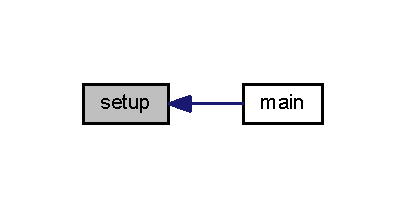
\includegraphics[width=195pt]{_project_main_8cpp_a4fc01d736fe50cf5b977f755b675f11d_icgraph}
\end{center}
\end{figure}


\hypertarget{_project_main_8cpp_acf0bcd0e759358b9284f65e0a55bc193}{}\index{Project\+Main.\+cpp@{Project\+Main.\+cpp}!task1000ms@{task1000ms}}
\index{task1000ms@{task1000ms}!Project\+Main.\+cpp@{Project\+Main.\+cpp}}
\subsubsection[{task1000ms(void)}]{\setlength{\rightskip}{0pt plus 5cm}void task1000ms (
\begin{DoxyParamCaption}
\item[{void}]{}
\end{DoxyParamCaption}
)}\label{_project_main_8cpp_acf0bcd0e759358b9284f65e0a55bc193}


Implementation of function that handle the 1000ms requests. 

Function declaration for tasks which are executed every 1000ms Function declaration for tasks which are executed every 1000ms Alternatively, you can use \#\+Box\+\_\+\+The\+\_\+\+Function\+\_\+\+Name.

Implementation of function that handle the 1000ms requests \begin{DoxyReturn}{Returns}
void 
\end{DoxyReturn}
\begin{DoxyNote}{Note}
Void function with no return. 
\end{DoxyNote}


Definition at line 187 of file Project\+Main.\+cpp.

\hypertarget{_project_main_8cpp_abc513c77d3ae6919b5983e6564643c11}{}\index{Project\+Main.\+cpp@{Project\+Main.\+cpp}!task100ms@{task100ms}}
\index{task100ms@{task100ms}!Project\+Main.\+cpp@{Project\+Main.\+cpp}}
\subsubsection[{task100ms(void)}]{\setlength{\rightskip}{0pt plus 5cm}void task100ms (
\begin{DoxyParamCaption}
\item[{void}]{}
\end{DoxyParamCaption}
)}\label{_project_main_8cpp_abc513c77d3ae6919b5983e6564643c11}


Implementation of function that handle the 100ms requests. 

Function declaration for tasks which are executed every 100ms Function declaration for tasks which are executed every 100ms Alternatively, you can use \#\+Box\+\_\+\+The\+\_\+\+Function\+\_\+\+Name.

Implementation of function that handle the 100ms requests \begin{DoxyReturn}{Returns}
void 
\end{DoxyReturn}
\begin{DoxyNote}{Note}
Void function with no return. 
\end{DoxyNote}


Definition at line 176 of file Project\+Main.\+cpp.

\hypertarget{_project_main_8cpp_aa0a2444ea9e75ec2a583b7e8a38560a6}{}\index{Project\+Main.\+cpp@{Project\+Main.\+cpp}!task20ms@{task20ms}}
\index{task20ms@{task20ms}!Project\+Main.\+cpp@{Project\+Main.\+cpp}}
\subsubsection[{task20ms(void)}]{\setlength{\rightskip}{0pt plus 5cm}void task20ms (
\begin{DoxyParamCaption}
\item[{void}]{}
\end{DoxyParamCaption}
)}\label{_project_main_8cpp_aa0a2444ea9e75ec2a583b7e8a38560a6}


Implementation of function that handle the 20ms requests. 

Function declaration for tasks which are executed every 20ms Function declaration for tasks which are executed every 20ms. Alternatively, you can use \#\+Box\+\_\+\+The\+\_\+\+Function\+\_\+\+Name.

Implementation of function that handle the 20ms requests \begin{DoxyReturn}{Returns}
void 
\end{DoxyReturn}
\begin{DoxyNote}{Note}
Void function with no return. 
\end{DoxyNote}


Definition at line 133 of file Project\+Main.\+cpp.



Here is the call graph for this function\+:\nopagebreak
\begin{figure}[H]
\begin{center}
\leavevmode
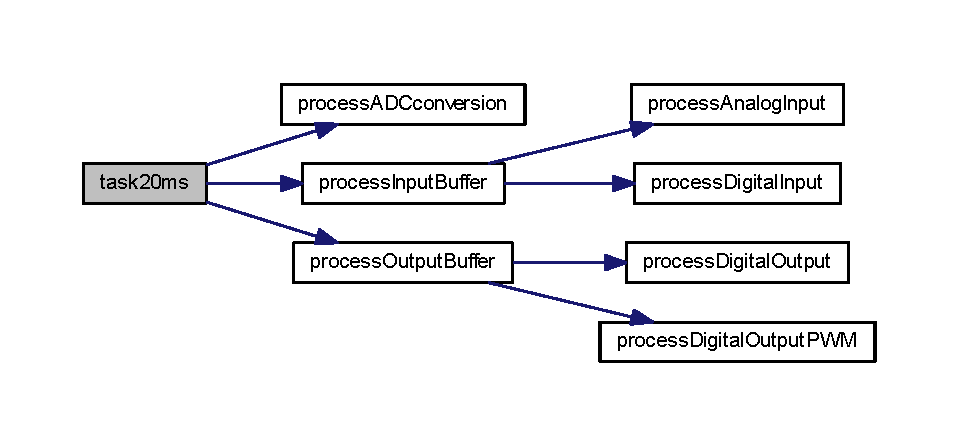
\includegraphics[width=350pt]{_project_main_8cpp_aa0a2444ea9e75ec2a583b7e8a38560a6_cgraph}
\end{center}
\end{figure}


\hypertarget{_project_main_8cpp_aca27d12738aa55893e5242ed21ab789c}{}\index{Project\+Main.\+cpp@{Project\+Main.\+cpp}!task40ms@{task40ms}}
\index{task40ms@{task40ms}!Project\+Main.\+cpp@{Project\+Main.\+cpp}}
\subsubsection[{task40ms(void)}]{\setlength{\rightskip}{0pt plus 5cm}void task40ms (
\begin{DoxyParamCaption}
\item[{void}]{}
\end{DoxyParamCaption}
)}\label{_project_main_8cpp_aca27d12738aa55893e5242ed21ab789c}


Implementation of function that handle the 40ms requests. 

Function declaration for tasks which are executed every40ms Function declaration for tasks which are executed every 40ms Alternatively, you can use \#\+Box\+\_\+\+The\+\_\+\+Function\+\_\+\+Name.

Implementation of function that handle the 40ms requests \begin{DoxyReturn}{Returns}
void 
\end{DoxyReturn}
\begin{DoxyNote}{Note}
Void function with no return. 
\end{DoxyNote}


Definition at line 150 of file Project\+Main.\+cpp.

\hypertarget{_project_main_8cpp_ada995e88886fe969d52c9f551201f7bc}{}\index{Project\+Main.\+cpp@{Project\+Main.\+cpp}!task60ms@{task60ms}}
\index{task60ms@{task60ms}!Project\+Main.\+cpp@{Project\+Main.\+cpp}}
\subsubsection[{task60ms(void)}]{\setlength{\rightskip}{0pt plus 5cm}void task60ms (
\begin{DoxyParamCaption}
\item[{void}]{}
\end{DoxyParamCaption}
)}\label{_project_main_8cpp_ada995e88886fe969d52c9f551201f7bc}


Implementation of function that handle the 60ms requests. 

Function declaration for tasks which are executed every 60ms Function declaration for tasks which are executed every 60ms. Alternatively, you can use \#\+Box\+\_\+\+The\+\_\+\+Function\+\_\+\+Name.

Implementation of function that handle the 60ms requests \begin{DoxyReturn}{Returns}
void 
\end{DoxyReturn}
\begin{DoxyNote}{Note}
Void function with no return. 
\end{DoxyNote}


Definition at line 165 of file Project\+Main.\+cpp.

\hypertarget{_project_main_8cpp_a612f7225aba66da17398c5472584559d}{}\index{Project\+Main.\+cpp@{Project\+Main.\+cpp}!task\+Get\+Config\+Ptr@{task\+Get\+Config\+Ptr}}
\index{task\+Get\+Config\+Ptr@{task\+Get\+Config\+Ptr}!Project\+Main.\+cpp@{Project\+Main.\+cpp}}
\subsubsection[{task\+Get\+Config\+Ptr(void)}]{\setlength{\rightskip}{0pt plus 5cm}{\bf Task\+Type\+\_\+st\+Type}$\ast$ task\+Get\+Config\+Ptr (
\begin{DoxyParamCaption}
\item[{void}]{}
\end{DoxyParamCaption}
)}\label{_project_main_8cpp_a612f7225aba66da17398c5472584559d}


Implementation of the function that returns a pointer to the tasks array. 

\begin{DoxyReturn}{Returns}
A pointer to the array of tasks 
\end{DoxyReturn}
\begin{DoxySeeAlso}{See also}
tasks\+\_\+st\mbox{[}\mbox{]}; 
\end{DoxySeeAlso}


Definition at line 70 of file Project\+Main.\+cpp.



Here is the caller graph for this function\+:\nopagebreak
\begin{figure}[H]
\begin{center}
\leavevmode
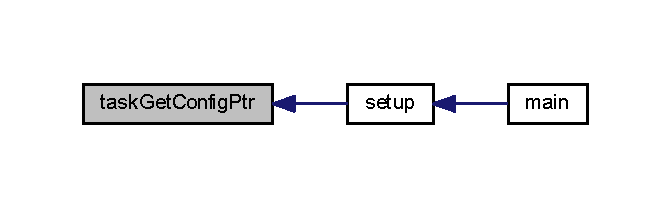
\includegraphics[width=322pt]{_project_main_8cpp_a612f7225aba66da17398c5472584559d_icgraph}
\end{center}
\end{figure}


\hypertarget{_project_main_8cpp_a99eb04bf8fed2beecfb3cb74451416c5}{}\index{Project\+Main.\+cpp@{Project\+Main.\+cpp}!timer0\+\_\+init@{timer0\+\_\+init}}
\index{timer0\+\_\+init@{timer0\+\_\+init}!Project\+Main.\+cpp@{Project\+Main.\+cpp}}
\subsubsection[{timer0\+\_\+init()}]{\setlength{\rightskip}{0pt plus 5cm}void timer0\+\_\+init (
\begin{DoxyParamCaption}
{}
\end{DoxyParamCaption}
)}\label{_project_main_8cpp_a99eb04bf8fed2beecfb3cb74451416c5}


Implementation of the function that initialize the timer0. 

Implementation of the function that initialize the timer 0 used in A\+D\+C conversion \begin{DoxyReturn}{Returns}
void 
\end{DoxyReturn}
$<$ digital pin6 is an output for lowbeam

$<$Clear O\+C0\+A on Compare Match

$<$enable interrupt on compare

$<$ sets the prescaler to 1024; 

Definition at line 198 of file Project\+Main.\+cpp.



Here is the caller graph for this function\+:\nopagebreak
\begin{figure}[H]
\begin{center}
\leavevmode
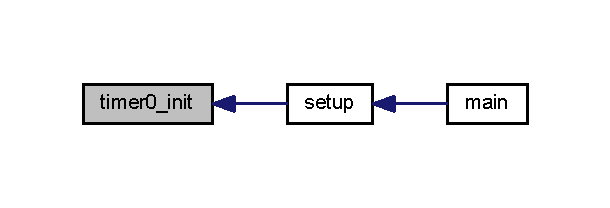
\includegraphics[width=293pt]{_project_main_8cpp_a99eb04bf8fed2beecfb3cb74451416c5_icgraph}
\end{center}
\end{figure}


\hypertarget{_project_main_8cpp_abb302081b7dbd40d0fea4bbe53fd9b7b}{}\index{Project\+Main.\+cpp@{Project\+Main.\+cpp}!timer1\+\_\+init@{timer1\+\_\+init}}
\index{timer1\+\_\+init@{timer1\+\_\+init}!Project\+Main.\+cpp@{Project\+Main.\+cpp}}
\subsubsection[{timer1\+\_\+init()}]{\setlength{\rightskip}{0pt plus 5cm}void timer1\+\_\+init (
\begin{DoxyParamCaption}
{}
\end{DoxyParamCaption}
)}\label{_project_main_8cpp_abb302081b7dbd40d0fea4bbe53fd9b7b}


Implementation of the function that initialize the timer1. 

Function definition for timer initialization Function implementation for timer initialization. Alternatively, you can use \#\+Box\+\_\+\+The\+\_\+\+Function\+\_\+\+Name.

Implementation of the function that initialize the timer 1 \begin{DoxyReturn}{Returns}
void 
\end{DoxyReturn}


Definition at line 214 of file Project\+Main.\+cpp.



Here is the caller graph for this function\+:\nopagebreak
\begin{figure}[H]
\begin{center}
\leavevmode
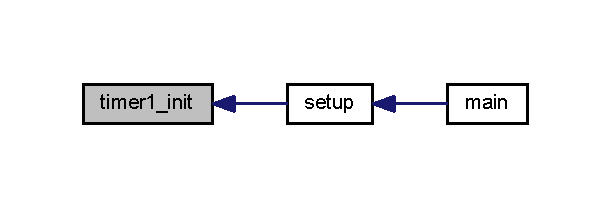
\includegraphics[width=293pt]{_project_main_8cpp_abb302081b7dbd40d0fea4bbe53fd9b7b_icgraph}
\end{center}
\end{figure}




\subsection{Variable Documentation}
\hypertarget{_project_main_8cpp_a364618e091f6af2a4ee81e8a38f2f974}{}\index{Project\+Main.\+cpp@{Project\+Main.\+cpp}!cui\+\_\+number\+Of\+Tasks@{cui\+\_\+number\+Of\+Tasks}}
\index{cui\+\_\+number\+Of\+Tasks@{cui\+\_\+number\+Of\+Tasks}!Project\+Main.\+cpp@{Project\+Main.\+cpp}}
\subsubsection[{cui\+\_\+number\+Of\+Tasks}]{\setlength{\rightskip}{0pt plus 5cm}const uint8\+\_\+t cui\+\_\+number\+Of\+Tasks = {\bf get\+Nr\+Tasks}()}\label{_project_main_8cpp_a364618e091f6af2a4ee81e8a38f2f974}


Definition at line 87 of file Project\+Main.\+cpp.

\hypertarget{_project_main_8cpp_ad626e67a0337fbbad267d2ea8187a995}{}\index{Project\+Main.\+cpp@{Project\+Main.\+cpp}!stui\+\_\+\+Task\+Index@{stui\+\_\+\+Task\+Index}}
\index{stui\+\_\+\+Task\+Index@{stui\+\_\+\+Task\+Index}!Project\+Main.\+cpp@{Project\+Main.\+cpp}}
\subsubsection[{stui\+\_\+\+Task\+Index}]{\setlength{\rightskip}{0pt plus 5cm}uint8\+\_\+t stui\+\_\+\+Task\+Index}\label{_project_main_8cpp_ad626e67a0337fbbad267d2ea8187a995}


Definition at line 84 of file Project\+Main.\+cpp.

\hypertarget{_project_main_8cpp_aef920dc87f0a96b97b10da1251f9d821}{}\index{Project\+Main.\+cpp@{Project\+Main.\+cpp}!task\+Time\+Counter\+\_\+u8@{task\+Time\+Counter\+\_\+u8}}
\index{task\+Time\+Counter\+\_\+u8@{task\+Time\+Counter\+\_\+u8}!Project\+Main.\+cpp@{Project\+Main.\+cpp}}
\subsubsection[{task\+Time\+Counter\+\_\+u8}]{\setlength{\rightskip}{0pt plus 5cm}volatile uint8\+\_\+t task\+Time\+Counter\+\_\+u8}\label{_project_main_8cpp_aef920dc87f0a96b97b10da1251f9d821}


Definition at line 86 of file Project\+Main.\+cpp.

\hypertarget{_project_main_8cpp_a771478af671521a8cc845b8efbf0855e}{}\index{Project\+Main.\+cpp@{Project\+Main.\+cpp}!task\+Time\+Counter\+Flag\+\_\+u8@{task\+Time\+Counter\+Flag\+\_\+u8}}
\index{task\+Time\+Counter\+Flag\+\_\+u8@{task\+Time\+Counter\+Flag\+\_\+u8}!Project\+Main.\+cpp@{Project\+Main.\+cpp}}
\subsubsection[{task\+Time\+Counter\+Flag\+\_\+u8}]{\setlength{\rightskip}{0pt plus 5cm}volatile uint8\+\_\+t task\+Time\+Counter\+Flag\+\_\+u8}\label{_project_main_8cpp_a771478af671521a8cc845b8efbf0855e}


Definition at line 85 of file Project\+Main.\+cpp.


\hypertarget{_project_main_8h}{}\section{Arduino\+U\+N\+O/src/\+Project\+Files/\+Project\+Main.h File Reference}
\label{_project_main_8h}\index{Arduino\+U\+N\+O/src/\+Project\+Files/\+Project\+Main.\+h@{Arduino\+U\+N\+O/src/\+Project\+Files/\+Project\+Main.\+h}}
{\ttfamily \#include $<$Arduino.\+h$>$}\\*
{\ttfamily \#include $<$Hardware\+Serial.\+h$>$}\\*
Include dependency graph for Project\+Main.\+h\+:
\nopagebreak
\begin{figure}[H]
\begin{center}
\leavevmode
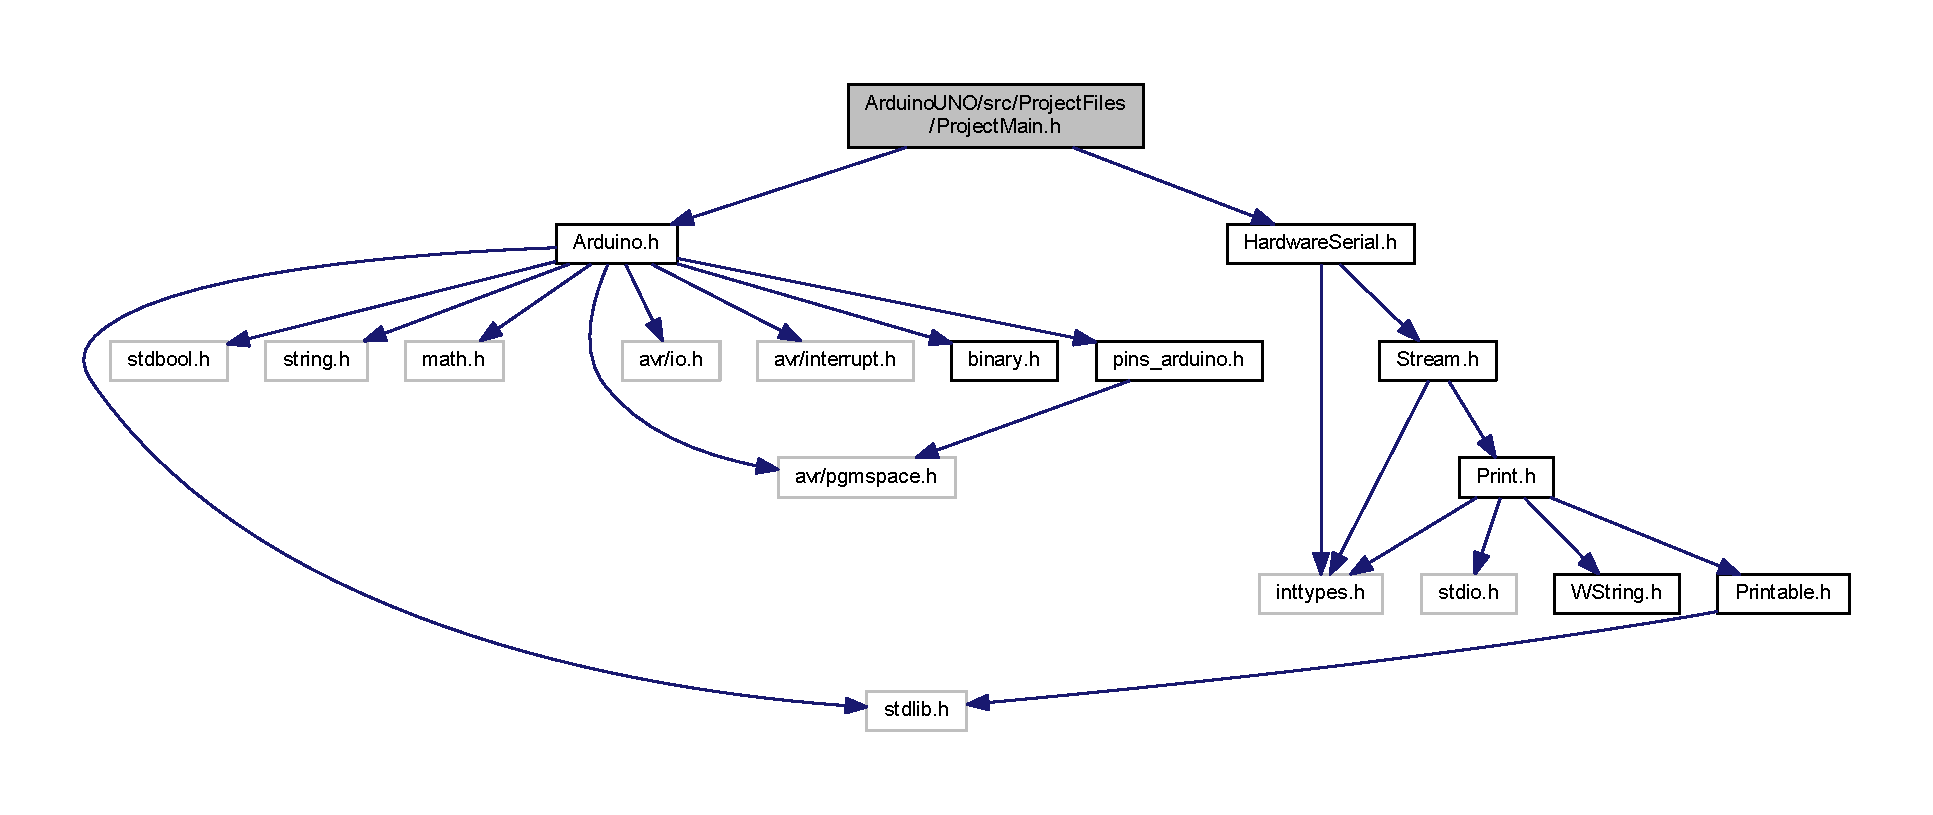
\includegraphics[width=350pt]{_project_main_8h__incl}
\end{center}
\end{figure}
This graph shows which files directly or indirectly include this file\+:
\nopagebreak
\begin{figure}[H]
\begin{center}
\leavevmode
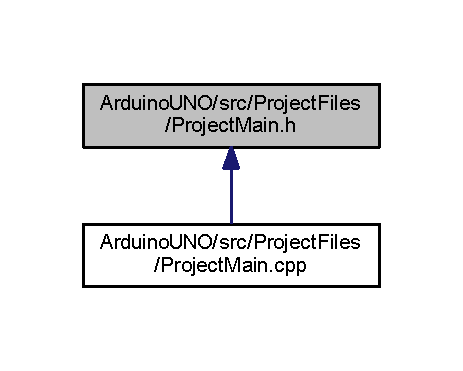
\includegraphics[width=222pt]{_project_main_8h__dep__incl}
\end{center}
\end{figure}
\subsection*{Macros}
\begin{DoxyCompactItemize}
\item 
\#define \hyperlink{_project_main_8h_a27a05420b36346cf71496473528b713c}{A\+R\+D\+U\+I\+N\+O\+\_\+\+M\+A\+I\+N}
\end{DoxyCompactItemize}
\subsection*{Functions}
\begin{DoxyCompactItemize}
\item 
void \hyperlink{_project_main_8h_aa0a2444ea9e75ec2a583b7e8a38560a6}{task20ms} (void)
\begin{DoxyCompactList}\small\item\em Function declaration for tasks which are executed every 20ms Function declaration for tasks which are executed every 20ms. Alternatively, you can use \#\+Box\+\_\+\+The\+\_\+\+Function\+\_\+\+Name. \end{DoxyCompactList}\item 
void \hyperlink{_project_main_8h_aca27d12738aa55893e5242ed21ab789c}{task40ms} (void)
\begin{DoxyCompactList}\small\item\em Function declaration for tasks which are executed every40ms Function declaration for tasks which are executed every 40ms Alternatively, you can use \#\+Box\+\_\+\+The\+\_\+\+Function\+\_\+\+Name. \end{DoxyCompactList}\item 
void \hyperlink{_project_main_8h_ada995e88886fe969d52c9f551201f7bc}{task60ms} (void)
\begin{DoxyCompactList}\small\item\em Function declaration for tasks which are executed every 60ms Function declaration for tasks which are executed every 60ms. Alternatively, you can use \#\+Box\+\_\+\+The\+\_\+\+Function\+\_\+\+Name. \end{DoxyCompactList}\item 
void \hyperlink{_project_main_8h_abc513c77d3ae6919b5983e6564643c11}{task100ms} (void)
\begin{DoxyCompactList}\small\item\em Function declaration for tasks which are executed every 100ms Function declaration for tasks which are executed every 100ms Alternatively, you can use \#\+Box\+\_\+\+The\+\_\+\+Function\+\_\+\+Name. \end{DoxyCompactList}\item 
void \hyperlink{_project_main_8h_acf0bcd0e759358b9284f65e0a55bc193}{task1000ms} (void)
\begin{DoxyCompactList}\small\item\em Function declaration for tasks which are executed every 1000ms Function declaration for tasks which are executed every 1000ms Alternatively, you can use \#\+Box\+\_\+\+The\+\_\+\+Function\+\_\+\+Name. \end{DoxyCompactList}\item 
void \hyperlink{_project_main_8h_a99eb04bf8fed2beecfb3cb74451416c5}{timer0\+\_\+init} ()
\begin{DoxyCompactList}\small\item\em Implementation of the function that initialize the timer0. \end{DoxyCompactList}\item 
void \hyperlink{_project_main_8h_abb302081b7dbd40d0fea4bbe53fd9b7b}{timer1\+\_\+init} ()
\begin{DoxyCompactList}\small\item\em Function definition for timer initialization Function implementation for timer initialization. Alternatively, you can use \#\+Box\+\_\+\+The\+\_\+\+Function\+\_\+\+Name. \end{DoxyCompactList}\end{DoxyCompactItemize}


\subsection{Macro Definition Documentation}
\hypertarget{_project_main_8h_a27a05420b36346cf71496473528b713c}{}\index{Project\+Main.\+h@{Project\+Main.\+h}!A\+R\+D\+U\+I\+N\+O\+\_\+\+M\+A\+I\+N@{A\+R\+D\+U\+I\+N\+O\+\_\+\+M\+A\+I\+N}}
\index{A\+R\+D\+U\+I\+N\+O\+\_\+\+M\+A\+I\+N@{A\+R\+D\+U\+I\+N\+O\+\_\+\+M\+A\+I\+N}!Project\+Main.\+h@{Project\+Main.\+h}}
\subsubsection[{A\+R\+D\+U\+I\+N\+O\+\_\+\+M\+A\+I\+N}]{\setlength{\rightskip}{0pt plus 5cm}\#define A\+R\+D\+U\+I\+N\+O\+\_\+\+M\+A\+I\+N}\label{_project_main_8h_a27a05420b36346cf71496473528b713c}


Definition at line 15 of file Project\+Main.\+h.



\subsection{Function Documentation}
\hypertarget{_project_main_8h_acf0bcd0e759358b9284f65e0a55bc193}{}\index{Project\+Main.\+h@{Project\+Main.\+h}!task1000ms@{task1000ms}}
\index{task1000ms@{task1000ms}!Project\+Main.\+h@{Project\+Main.\+h}}
\subsubsection[{task1000ms(void)}]{\setlength{\rightskip}{0pt plus 5cm}void task1000ms (
\begin{DoxyParamCaption}
\item[{void}]{}
\end{DoxyParamCaption}
)}\label{_project_main_8h_acf0bcd0e759358b9284f65e0a55bc193}


Function declaration for tasks which are executed every 1000ms Function declaration for tasks which are executed every 1000ms Alternatively, you can use \#\+Box\+\_\+\+The\+\_\+\+Function\+\_\+\+Name. 

\begin{DoxyReturn}{Returns}
void
\end{DoxyReturn}
Function declaration for tasks which are executed every 1000ms Function declaration for tasks which are executed every 1000ms Alternatively, you can use \#\+Box\+\_\+\+The\+\_\+\+Function\+\_\+\+Name.

Implementation of function that handle the 1000ms requests \begin{DoxyReturn}{Returns}
void 
\end{DoxyReturn}
\begin{DoxyNote}{Note}
Void function with no return. 
\end{DoxyNote}


Definition at line 187 of file Project\+Main.\+cpp.

\hypertarget{_project_main_8h_abc513c77d3ae6919b5983e6564643c11}{}\index{Project\+Main.\+h@{Project\+Main.\+h}!task100ms@{task100ms}}
\index{task100ms@{task100ms}!Project\+Main.\+h@{Project\+Main.\+h}}
\subsubsection[{task100ms(void)}]{\setlength{\rightskip}{0pt plus 5cm}void task100ms (
\begin{DoxyParamCaption}
\item[{void}]{}
\end{DoxyParamCaption}
)}\label{_project_main_8h_abc513c77d3ae6919b5983e6564643c11}


Function declaration for tasks which are executed every 100ms Function declaration for tasks which are executed every 100ms Alternatively, you can use \#\+Box\+\_\+\+The\+\_\+\+Function\+\_\+\+Name. 

\begin{DoxyReturn}{Returns}
void
\end{DoxyReturn}
Function declaration for tasks which are executed every 100ms Function declaration for tasks which are executed every 100ms Alternatively, you can use \#\+Box\+\_\+\+The\+\_\+\+Function\+\_\+\+Name.

Implementation of function that handle the 100ms requests \begin{DoxyReturn}{Returns}
void 
\end{DoxyReturn}
\begin{DoxyNote}{Note}
Void function with no return. 
\end{DoxyNote}


Definition at line 176 of file Project\+Main.\+cpp.

\hypertarget{_project_main_8h_aa0a2444ea9e75ec2a583b7e8a38560a6}{}\index{Project\+Main.\+h@{Project\+Main.\+h}!task20ms@{task20ms}}
\index{task20ms@{task20ms}!Project\+Main.\+h@{Project\+Main.\+h}}
\subsubsection[{task20ms(void)}]{\setlength{\rightskip}{0pt plus 5cm}void task20ms (
\begin{DoxyParamCaption}
\item[{void}]{}
\end{DoxyParamCaption}
)}\label{_project_main_8h_aa0a2444ea9e75ec2a583b7e8a38560a6}


Function declaration for tasks which are executed every 20ms Function declaration for tasks which are executed every 20ms. Alternatively, you can use \#\+Box\+\_\+\+The\+\_\+\+Function\+\_\+\+Name. 

\begin{DoxyReturn}{Returns}
void
\end{DoxyReturn}
Function declaration for tasks which are executed every 20ms Function declaration for tasks which are executed every 20ms. Alternatively, you can use \#\+Box\+\_\+\+The\+\_\+\+Function\+\_\+\+Name.

Implementation of function that handle the 20ms requests \begin{DoxyReturn}{Returns}
void 
\end{DoxyReturn}
\begin{DoxyNote}{Note}
Void function with no return. 
\end{DoxyNote}


Definition at line 133 of file Project\+Main.\+cpp.



Here is the call graph for this function\+:
\nopagebreak
\begin{figure}[H]
\begin{center}
\leavevmode
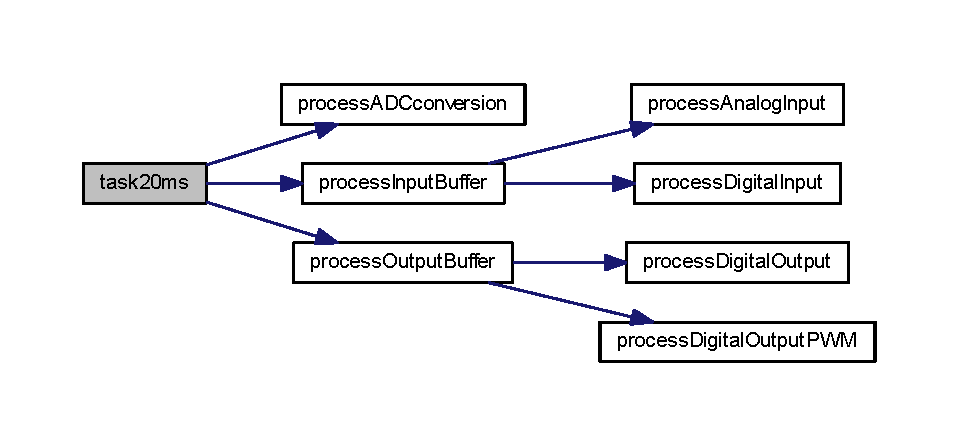
\includegraphics[width=350pt]{_project_main_8h_aa0a2444ea9e75ec2a583b7e8a38560a6_cgraph}
\end{center}
\end{figure}


\hypertarget{_project_main_8h_aca27d12738aa55893e5242ed21ab789c}{}\index{Project\+Main.\+h@{Project\+Main.\+h}!task40ms@{task40ms}}
\index{task40ms@{task40ms}!Project\+Main.\+h@{Project\+Main.\+h}}
\subsubsection[{task40ms(void)}]{\setlength{\rightskip}{0pt plus 5cm}void task40ms (
\begin{DoxyParamCaption}
\item[{void}]{}
\end{DoxyParamCaption}
)}\label{_project_main_8h_aca27d12738aa55893e5242ed21ab789c}


Function declaration for tasks which are executed every40ms Function declaration for tasks which are executed every 40ms Alternatively, you can use \#\+Box\+\_\+\+The\+\_\+\+Function\+\_\+\+Name. 

\begin{DoxyReturn}{Returns}
void
\end{DoxyReturn}
Function declaration for tasks which are executed every40ms Function declaration for tasks which are executed every 40ms Alternatively, you can use \#\+Box\+\_\+\+The\+\_\+\+Function\+\_\+\+Name.

Implementation of function that handle the 40ms requests \begin{DoxyReturn}{Returns}
void 
\end{DoxyReturn}
\begin{DoxyNote}{Note}
Void function with no return. 
\end{DoxyNote}


Definition at line 150 of file Project\+Main.\+cpp.

\hypertarget{_project_main_8h_ada995e88886fe969d52c9f551201f7bc}{}\index{Project\+Main.\+h@{Project\+Main.\+h}!task60ms@{task60ms}}
\index{task60ms@{task60ms}!Project\+Main.\+h@{Project\+Main.\+h}}
\subsubsection[{task60ms(void)}]{\setlength{\rightskip}{0pt plus 5cm}void task60ms (
\begin{DoxyParamCaption}
\item[{void}]{}
\end{DoxyParamCaption}
)}\label{_project_main_8h_ada995e88886fe969d52c9f551201f7bc}


Function declaration for tasks which are executed every 60ms Function declaration for tasks which are executed every 60ms. Alternatively, you can use \#\+Box\+\_\+\+The\+\_\+\+Function\+\_\+\+Name. 

\begin{DoxyReturn}{Returns}
void
\end{DoxyReturn}
Function declaration for tasks which are executed every 60ms Function declaration for tasks which are executed every 60ms. Alternatively, you can use \#\+Box\+\_\+\+The\+\_\+\+Function\+\_\+\+Name.

Implementation of function that handle the 60ms requests \begin{DoxyReturn}{Returns}
void 
\end{DoxyReturn}
\begin{DoxyNote}{Note}
Void function with no return. 
\end{DoxyNote}


Definition at line 165 of file Project\+Main.\+cpp.

\hypertarget{_project_main_8h_a99eb04bf8fed2beecfb3cb74451416c5}{}\index{Project\+Main.\+h@{Project\+Main.\+h}!timer0\+\_\+init@{timer0\+\_\+init}}
\index{timer0\+\_\+init@{timer0\+\_\+init}!Project\+Main.\+h@{Project\+Main.\+h}}
\subsubsection[{timer0\+\_\+init()}]{\setlength{\rightskip}{0pt plus 5cm}void timer0\+\_\+init (
\begin{DoxyParamCaption}
{}
\end{DoxyParamCaption}
)}\label{_project_main_8h_a99eb04bf8fed2beecfb3cb74451416c5}


Implementation of the function that initialize the timer0. 

H\+E\+A\+D Function prototype Initialize the timer0 for A\+D\+C conversion

Implementation of the function that initialize the timer 0 used in A\+D\+C conversion \begin{DoxyReturn}{Returns}
void 
\end{DoxyReturn}
$<$ digital pin6 is an output for lowbeam

$<$Clear O\+C0\+A on Compare Match

$<$enable interrupt on compare

$<$ sets the prescaler to 1024; 

Definition at line 198 of file Project\+Main.\+cpp.



Here is the caller graph for this function\+:
\nopagebreak
\begin{figure}[H]
\begin{center}
\leavevmode
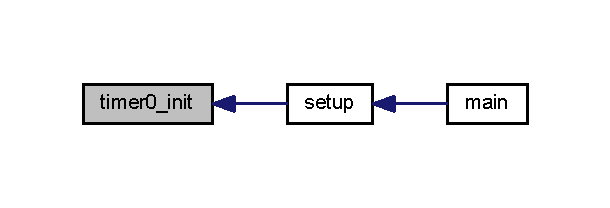
\includegraphics[width=293pt]{_project_main_8h_a99eb04bf8fed2beecfb3cb74451416c5_icgraph}
\end{center}
\end{figure}


\hypertarget{_project_main_8h_abb302081b7dbd40d0fea4bbe53fd9b7b}{}\index{Project\+Main.\+h@{Project\+Main.\+h}!timer1\+\_\+init@{timer1\+\_\+init}}
\index{timer1\+\_\+init@{timer1\+\_\+init}!Project\+Main.\+h@{Project\+Main.\+h}}
\subsubsection[{timer1\+\_\+init()}]{\setlength{\rightskip}{0pt plus 5cm}void timer1\+\_\+init (
\begin{DoxyParamCaption}
{}
\end{DoxyParamCaption}
)}\label{_project_main_8h_abb302081b7dbd40d0fea4bbe53fd9b7b}


Function definition for timer initialization Function implementation for timer initialization. Alternatively, you can use \#\+Box\+\_\+\+The\+\_\+\+Function\+\_\+\+Name. 

Function prototype \subsection*{Initialize the timer1 }

\begin{DoxyReturn}{Returns}
void \begin{quote}
\begin{quote}
\begin{quote}
\begin{quote}
\begin{quote}
\begin{quote}
\begin{quote}
558e0ec9797d9908c34a8d271e1e2aeb7cc47775\end{quote}
\end{quote}
\end{quote}
\end{quote}
\end{quote}
\end{quote}
\end{quote}

\end{DoxyReturn}
Function definition for timer initialization Function implementation for timer initialization. Alternatively, you can use \#\+Box\+\_\+\+The\+\_\+\+Function\+\_\+\+Name.

Implementation of the function that initialize the timer 1 \begin{DoxyReturn}{Returns}
void 
\end{DoxyReturn}


Definition at line 214 of file Project\+Main.\+cpp.



Here is the caller graph for this function\+:
\nopagebreak
\begin{figure}[H]
\begin{center}
\leavevmode
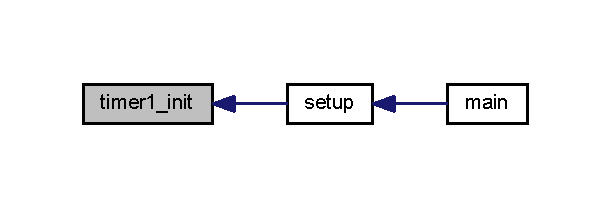
\includegraphics[width=293pt]{_project_main_8h_abb302081b7dbd40d0fea4bbe53fd9b7b_icgraph}
\end{center}
\end{figure}



\hypertarget{scheduler_config_8h}{}\section{Arduino\+U\+N\+O/src/\+Project\+Files/scheduler\+Config.h File Reference}
\label{scheduler_config_8h}\index{Arduino\+U\+N\+O/src/\+Project\+Files/scheduler\+Config.\+h@{Arduino\+U\+N\+O/src/\+Project\+Files/scheduler\+Config.\+h}}
This graph shows which files directly or indirectly include this file\+:
\nopagebreak
\begin{figure}[H]
\begin{center}
\leavevmode
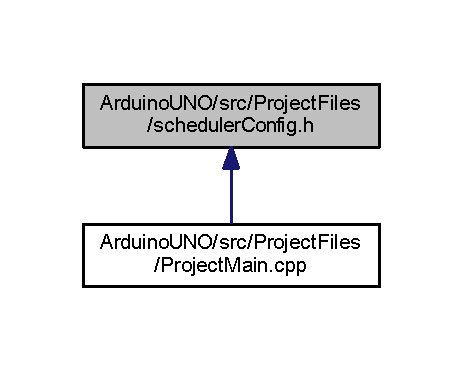
\includegraphics[width=222pt]{scheduler_config_8h__dep__incl}
\end{center}
\end{figure}
\subsection*{Data Structures}
\begin{DoxyCompactItemize}
\item 
struct \hyperlink{struct_task_type__st_type}{Task\+Type\+\_\+st\+Type}
\begin{DoxyCompactList}\small\item\em Structure used to define a task and the interval of the execution. \end{DoxyCompactList}\end{DoxyCompactItemize}
\subsection*{Macros}
\begin{DoxyCompactItemize}
\item 
\#define \hyperlink{scheduler_config_8h_a1e4a93d0aaa29bef43ca5eb4656c4034}{T\+\_\+\+I\+N\+T\+E\+R\+V\+A\+L\+\_\+20\+M\+S}~1
\item 
\#define \hyperlink{scheduler_config_8h_afc9dea09dea542ef25be5ef307e4b08e}{T\+\_\+\+I\+N\+T\+E\+R\+V\+A\+L\+\_\+40\+M\+S}~2
\item 
\#define \hyperlink{scheduler_config_8h_a7407d15e636723dd8ab5f7f6b83991c4}{T\+\_\+\+I\+N\+T\+E\+R\+V\+A\+L\+\_\+60\+M\+S}~3
\item 
\#define \hyperlink{scheduler_config_8h_a16d6c905fbc0f09edeafd4de45ea0c4c}{T\+\_\+\+I\+N\+T\+E\+R\+V\+A\+L\+\_\+100\+M\+S}~5
\item 
\#define \hyperlink{scheduler_config_8h_a36f3fe7246488b3e874975602560105a}{T\+\_\+\+I\+N\+T\+E\+R\+V\+A\+L\+\_\+1000\+M\+S}~50
\item 
\#define \hyperlink{scheduler_config_8h_ae3952bdeb41b7b6339b1f729d9c6f364}{T\+\_\+\+T\+I\+M\+E\+R\+\_\+\+S\+T\+A\+R\+T}~64286
\end{DoxyCompactItemize}


\subsection{Macro Definition Documentation}
\hypertarget{scheduler_config_8h_a36f3fe7246488b3e874975602560105a}{}\index{scheduler\+Config.\+h@{scheduler\+Config.\+h}!T\+\_\+\+I\+N\+T\+E\+R\+V\+A\+L\+\_\+1000\+M\+S@{T\+\_\+\+I\+N\+T\+E\+R\+V\+A\+L\+\_\+1000\+M\+S}}
\index{T\+\_\+\+I\+N\+T\+E\+R\+V\+A\+L\+\_\+1000\+M\+S@{T\+\_\+\+I\+N\+T\+E\+R\+V\+A\+L\+\_\+1000\+M\+S}!scheduler\+Config.\+h@{scheduler\+Config.\+h}}
\subsubsection[{T\+\_\+\+I\+N\+T\+E\+R\+V\+A\+L\+\_\+1000\+M\+S}]{\setlength{\rightskip}{0pt plus 5cm}\#define T\+\_\+\+I\+N\+T\+E\+R\+V\+A\+L\+\_\+1000\+M\+S~50}\label{scheduler_config_8h_a36f3fe7246488b3e874975602560105a}
The interval in ticks to call the 1000 ms tasks 

Definition at line 35 of file scheduler\+Config.\+h.

\hypertarget{scheduler_config_8h_a16d6c905fbc0f09edeafd4de45ea0c4c}{}\index{scheduler\+Config.\+h@{scheduler\+Config.\+h}!T\+\_\+\+I\+N\+T\+E\+R\+V\+A\+L\+\_\+100\+M\+S@{T\+\_\+\+I\+N\+T\+E\+R\+V\+A\+L\+\_\+100\+M\+S}}
\index{T\+\_\+\+I\+N\+T\+E\+R\+V\+A\+L\+\_\+100\+M\+S@{T\+\_\+\+I\+N\+T\+E\+R\+V\+A\+L\+\_\+100\+M\+S}!scheduler\+Config.\+h@{scheduler\+Config.\+h}}
\subsubsection[{T\+\_\+\+I\+N\+T\+E\+R\+V\+A\+L\+\_\+100\+M\+S}]{\setlength{\rightskip}{0pt plus 5cm}\#define T\+\_\+\+I\+N\+T\+E\+R\+V\+A\+L\+\_\+100\+M\+S~5}\label{scheduler_config_8h_a16d6c905fbc0f09edeafd4de45ea0c4c}
The interval in ticks to call the 100 ms tasks 

Definition at line 30 of file scheduler\+Config.\+h.

\hypertarget{scheduler_config_8h_a1e4a93d0aaa29bef43ca5eb4656c4034}{}\index{scheduler\+Config.\+h@{scheduler\+Config.\+h}!T\+\_\+\+I\+N\+T\+E\+R\+V\+A\+L\+\_\+20\+M\+S@{T\+\_\+\+I\+N\+T\+E\+R\+V\+A\+L\+\_\+20\+M\+S}}
\index{T\+\_\+\+I\+N\+T\+E\+R\+V\+A\+L\+\_\+20\+M\+S@{T\+\_\+\+I\+N\+T\+E\+R\+V\+A\+L\+\_\+20\+M\+S}!scheduler\+Config.\+h@{scheduler\+Config.\+h}}
\subsubsection[{T\+\_\+\+I\+N\+T\+E\+R\+V\+A\+L\+\_\+20\+M\+S}]{\setlength{\rightskip}{0pt plus 5cm}\#define T\+\_\+\+I\+N\+T\+E\+R\+V\+A\+L\+\_\+20\+M\+S~1}\label{scheduler_config_8h_a1e4a93d0aaa29bef43ca5eb4656c4034}
The interval in ticks to call the 20 ms tasks 

Definition at line 15 of file scheduler\+Config.\+h.

\hypertarget{scheduler_config_8h_afc9dea09dea542ef25be5ef307e4b08e}{}\index{scheduler\+Config.\+h@{scheduler\+Config.\+h}!T\+\_\+\+I\+N\+T\+E\+R\+V\+A\+L\+\_\+40\+M\+S@{T\+\_\+\+I\+N\+T\+E\+R\+V\+A\+L\+\_\+40\+M\+S}}
\index{T\+\_\+\+I\+N\+T\+E\+R\+V\+A\+L\+\_\+40\+M\+S@{T\+\_\+\+I\+N\+T\+E\+R\+V\+A\+L\+\_\+40\+M\+S}!scheduler\+Config.\+h@{scheduler\+Config.\+h}}
\subsubsection[{T\+\_\+\+I\+N\+T\+E\+R\+V\+A\+L\+\_\+40\+M\+S}]{\setlength{\rightskip}{0pt plus 5cm}\#define T\+\_\+\+I\+N\+T\+E\+R\+V\+A\+L\+\_\+40\+M\+S~2}\label{scheduler_config_8h_afc9dea09dea542ef25be5ef307e4b08e}
The interval in ticks to call the 40 ms tasks 

Definition at line 20 of file scheduler\+Config.\+h.

\hypertarget{scheduler_config_8h_a7407d15e636723dd8ab5f7f6b83991c4}{}\index{scheduler\+Config.\+h@{scheduler\+Config.\+h}!T\+\_\+\+I\+N\+T\+E\+R\+V\+A\+L\+\_\+60\+M\+S@{T\+\_\+\+I\+N\+T\+E\+R\+V\+A\+L\+\_\+60\+M\+S}}
\index{T\+\_\+\+I\+N\+T\+E\+R\+V\+A\+L\+\_\+60\+M\+S@{T\+\_\+\+I\+N\+T\+E\+R\+V\+A\+L\+\_\+60\+M\+S}!scheduler\+Config.\+h@{scheduler\+Config.\+h}}
\subsubsection[{T\+\_\+\+I\+N\+T\+E\+R\+V\+A\+L\+\_\+60\+M\+S}]{\setlength{\rightskip}{0pt plus 5cm}\#define T\+\_\+\+I\+N\+T\+E\+R\+V\+A\+L\+\_\+60\+M\+S~3}\label{scheduler_config_8h_a7407d15e636723dd8ab5f7f6b83991c4}
The interval in ticks to call the 60 ms tasks 

Definition at line 25 of file scheduler\+Config.\+h.

\hypertarget{scheduler_config_8h_ae3952bdeb41b7b6339b1f729d9c6f364}{}\index{scheduler\+Config.\+h@{scheduler\+Config.\+h}!T\+\_\+\+T\+I\+M\+E\+R\+\_\+\+S\+T\+A\+R\+T@{T\+\_\+\+T\+I\+M\+E\+R\+\_\+\+S\+T\+A\+R\+T}}
\index{T\+\_\+\+T\+I\+M\+E\+R\+\_\+\+S\+T\+A\+R\+T@{T\+\_\+\+T\+I\+M\+E\+R\+\_\+\+S\+T\+A\+R\+T}!scheduler\+Config.\+h@{scheduler\+Config.\+h}}
\subsubsection[{T\+\_\+\+T\+I\+M\+E\+R\+\_\+\+S\+T\+A\+R\+T}]{\setlength{\rightskip}{0pt plus 5cm}\#define T\+\_\+\+T\+I\+M\+E\+R\+\_\+\+S\+T\+A\+R\+T~64286}\label{scheduler_config_8h_ae3952bdeb41b7b6339b1f729d9c6f364}
The start value of the Timer 

Definition at line 41 of file scheduler\+Config.\+h.


%--- End generated contents ---

% Index
\backmatter
\newpage
\phantomsection
\clearemptydoublepage
\addcontentsline{toc}{chapter}{Index}
\printindex

\end{document}
